\chapter{Installation}
\label{chapter:Installation}

\index{Installation}

This section describes the process for installing ITK on your system. Keep in
mind that ITK is a toolkit, and as such, once it is installed in your computer
there will be no application to run. Rather, use ITK to build your own
applications. What ITK does provide---besides the toolkit proper---is a large
set of test files and examples that will introduce ITK concepts and will show
how to use ITK in your own projects.

Some of the examples distributed with ITK require third party libraries that
may require installation. For an initial installation of ITK, you may want to
ignore these extra libraries and just build the toolkit itself.

ITK has been developed and tested across different combinations of
operating systems, compilers, and hardware platforms including
Microsoft Windows, Linux on various architectures, Solaris, Mac
OSX, and Cygwin.  It is known to work with the following compilers:

%TODO Need to update this list
\begin{itemize}
\item GCC 4.x
\item Visual Studio 8 SP 1 (Until 2015), 9 (Until 2018), 10 (Until 2020)
\item Intel Compiler Suite 11.x, 12.x
\item Darwin-c++-4.2 PPC (Until 2015), x86\_64
\item Win32-mingw-gcc-4.5
\item Clang 3.3 and later
\end{itemize}

Support for different platforms is evident on the ITK quality dashboard
(see Section \ref{sec:CDash} on page \pageref{sec:CDash}).

Given the advanced usage of C++ features in the toolkit, some
compilers may have difficulties processing the code. If you are
currently using an outdated compiler this may be an excellent excuse
for upgrading this old piece of software!

\section{Building ITK}
\label{sec:Build ITK}

\index{Build}

The challenge of supporting ITK across platforms has been solved through the
use of CMake\footnote{\url{www.cmake.org}}, a cross-platform, open-source build system.
CMake is used to control the software compilation process using simple platform
and compiler independent configuration files.  CMake generates native makefiles
and workspaces that can be used in the compiler environment of your choice.
CMake is quite sophisticated---it supports complex environments requiring
system introspection, compiler feature testing, and code generation.

CMake generates Makefiles under UNIX and Cygwin systems and generates Visual
Studio workspaces under Windows (and appropriate build files for other systems
like Eclipse). The information used by CMake is provided by
\code{CMakeLists.txt} files that are present in every directory of the ITK
source tree. These files contain information that the user provides to CMake
at configuration time. Typical information includes paths to utilities in the
system and the selection of software options specified by the user.

An ITK build requires only CMake and a C++ compiler. ITK ships with all the
third party library dependencies required, and these will be used unless the
use of a system version is requested during CMake configuration.

\subsection{Preparing CMake}
\label{sec:CMakeforITK}

\index{CMake}
\index{CMake!downloading}

CMake can be downloaded at no cost from
\begin{center}
  \url{http://www.cmake.org/cmake/resources/software.html}
\end{center}

The mininum version of CMake has been evolving along with the version of ITK.
For example, the current latest version of ITK (\ITKVERSIONMAJORMINOR)
requires the minimum CMake version to be 2.8.8. You can download binary
versions for most of the popular platforms including Windows, Solaris, HP, Mac
and Linux. Alternatively you can download the source code and build CMake on
your system. Follow the instructions in the CMake web page for downloading and
installing the software.

Running CMake initially requires that you provide two pieces of information:
where the source code directory is located (ITK\_SOURCE\_DIR), and where the
object code is to be produced (ITK\_BINARY\_DIR). These are referred to as the
\emph{source directory} and the \emph{binary directory}. We recommend setting
the binary directory to be different than the source directory (an
\emph{out-of-source} build).  On Unix, the binary directory is created by the
user and CMake is invoked with the path to the source directory. For example:

\small
\begin{verbatim}
mkdir ITK-build
cd ITK-build
ccmake ../ITK
\end{verbatim}
\normalsize

On Windows, the CMake GUI is used to specify the source and build
directories (Figure \ref{fig:CMakeGUI}).

CMake runs in an interactive mode in that you iteratively select options and
configure according to these options. The iteration proceeds until no more
options remain to be selected. At this point, a generation step produces the appropriate
build files for your configuration.

This interactive configuration process can be better understood if you
imagine that you are walking through a decision tree.  Every option that you
select introduces the possibility that new, dependent options may become
relevant. These new options are presented by CMake at the top of the options
list in its interface.  Only when no new options appear after a configuration
iteration can you be sure that the necessary decisions have all been made. At
this point build files are generated for the current configuration.

\subsection{Configuring ITK}
\label{sec:ConfigureITK}

\begin{figure}[htb!]
\centering
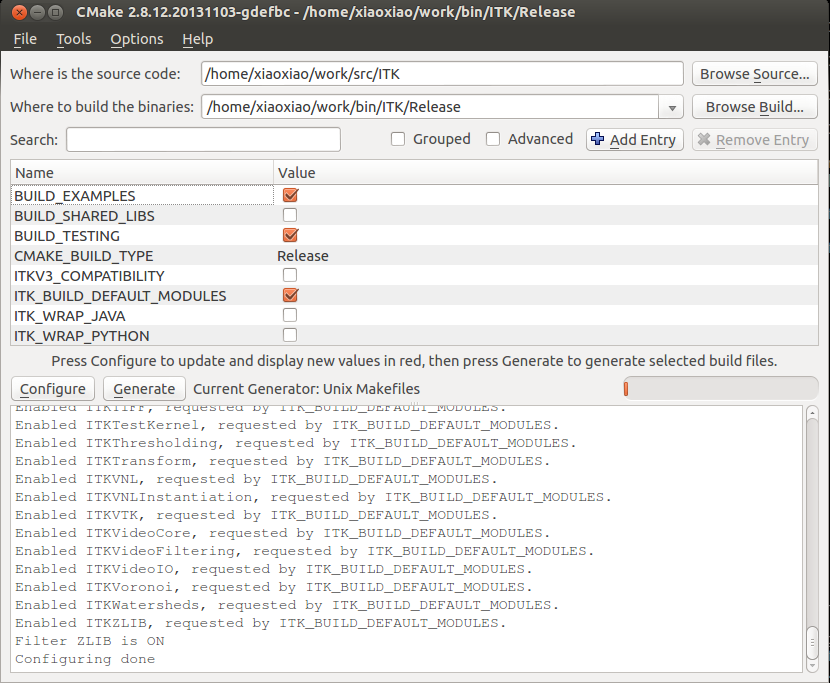
\includegraphics[width=0.8\textwidth]{ITK_CMake_GUI_Ubuntu.eps}
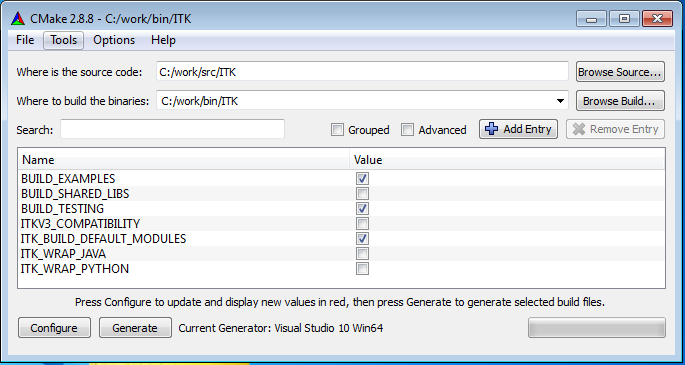
\includegraphics[width=0.8\textwidth]{ITK_CMake_GUI_Windows.eps}
\itkcaption[CMake user interface]{CMake interface. Top) \texttt{ccmake}, the UNIX
version based on \texttt{curses}. Bottom) \texttt{CMakeSetup}, the MS-Windows
version based on MFC.}
\label{fig:CMakeGUI}
\end{figure}

Figure \ref{fig:CMakeGUI} shows the CMake interface for UNIX and MS-Windows.
In order to speed up the build process, disable the compilation
of the unit tests and examples. This is done with the variables
\code{BUILD\_TESTING=OFF} and \code{BUILD\_EXAMPLES=OFF}.  The examples
distributed with the toolkit are a helpful resource for learning how to use ITK
components but are not essential for the use of the toolkit itself. The testing
section includes a large number of small programs that exercise the
capabilities of ITK classes. Due to the large number of tests, enabling the
testing option will considerably increase the build time.  It is not
desirable to enable this option for a first build of the toolkit.

Begin running CMake by using \code{ccmake} on Unix, and \code{CMakeSetup} on
Windows.  Remember to run \code{ccmake} from the binary directory on Unix. On
Windows, specify the source and binary directories in the GUI, then begin to
set the build variables in the GUI as necessary.  Most variables should have
default values that are sensible. Each time you change a set of variables in
CMake, it is necessary to proceed to another configuration step. In the
Windows version this is done by clicking on the ``Configure'' button. In the
UNIX version this is done in an interface using the curses library, where you
can configure by hitting the ``c'' key.

When no new options appear in CMake, you can proceed to generate Makefiles or
Visual Studio projects (or appropriate build file(s) depending on your
compiler). This is done in Windows by clicking on the ``Ok'' button.  In the
UNIX version this is done by hitting the ``g'' key. After the generation
process CMake will quit silently. To initiate the build process on UNIX,
simply type \code{make} in the binary directory. Under Windows, load the
workspace named \code{ITK.dsw} (if using MSDEV) or \code{ITK.sln} (if using
Visual Studio) from the binary directory specified in the CMake GUI.

The build process will typically take anywhere from 15 minutes to a couple of
hours depending on the the build configuration and the performance of your
system. If testing is enabled as part of the normal build process,
about 2400 test programs will be compiled. This will verify that all the
components of ITK have been correctly built on your system.


\subsection{Advanced Module Configuration}
\label{sec:ModuleConfiguration}
Following the default configuration introduced in \ref{sec:ConfigureITK},
the majority of the toolkit will be built. The modern modular structure of the
tookit makes it possible to customize the ITK library with choices of modules.
ITK was officially modularized in version 4.0.0 released in December of 2011.
Developers have been testing and improving the modular structure since then.
The toolkit currently contains 137 regular/internal modules, four remote
modules and counting.

By default, most internal ITK modules except the ones that depend on external
third party libraries (such as \code{ITKVtkGlue}, \code{ITKBridgeOpenCV},
\code{ITKBridgeVXL}, etc.) and several  modules with legacy code
(\code{ITKReview}, \code{ITKDeprecated} and \code{ITKv3Compatibility}),  will
be built into the ITK library. All non-default modules have
\code{EXCLUDE\_FROM\_DEFAULT} tag in their module definition file
(itk-module.cmake), including the remote modules.

\code{ITK\_BUILD\_DEFAULT\_MODULES} is the CMake option to request all the
default modules in the toolkit, by default this option is ON as shown in Figure
\ref{fig:CMakeGUI}.  In the advanced mode of the CMake GUI, you can manually
toggle those non-default modules via the \code{Module\_\{module name\}}
options.   All default modules’ \code{Module\_\{module name\}} options are not
available  for toggle since they are requested and enabled via
\code{ITK\_BUILD\_DEFAULT\_MODULES = ON} already, see Figure
\ref{fig:ConfigITKDefault}.

\begin{figure}[htb!]
\centering
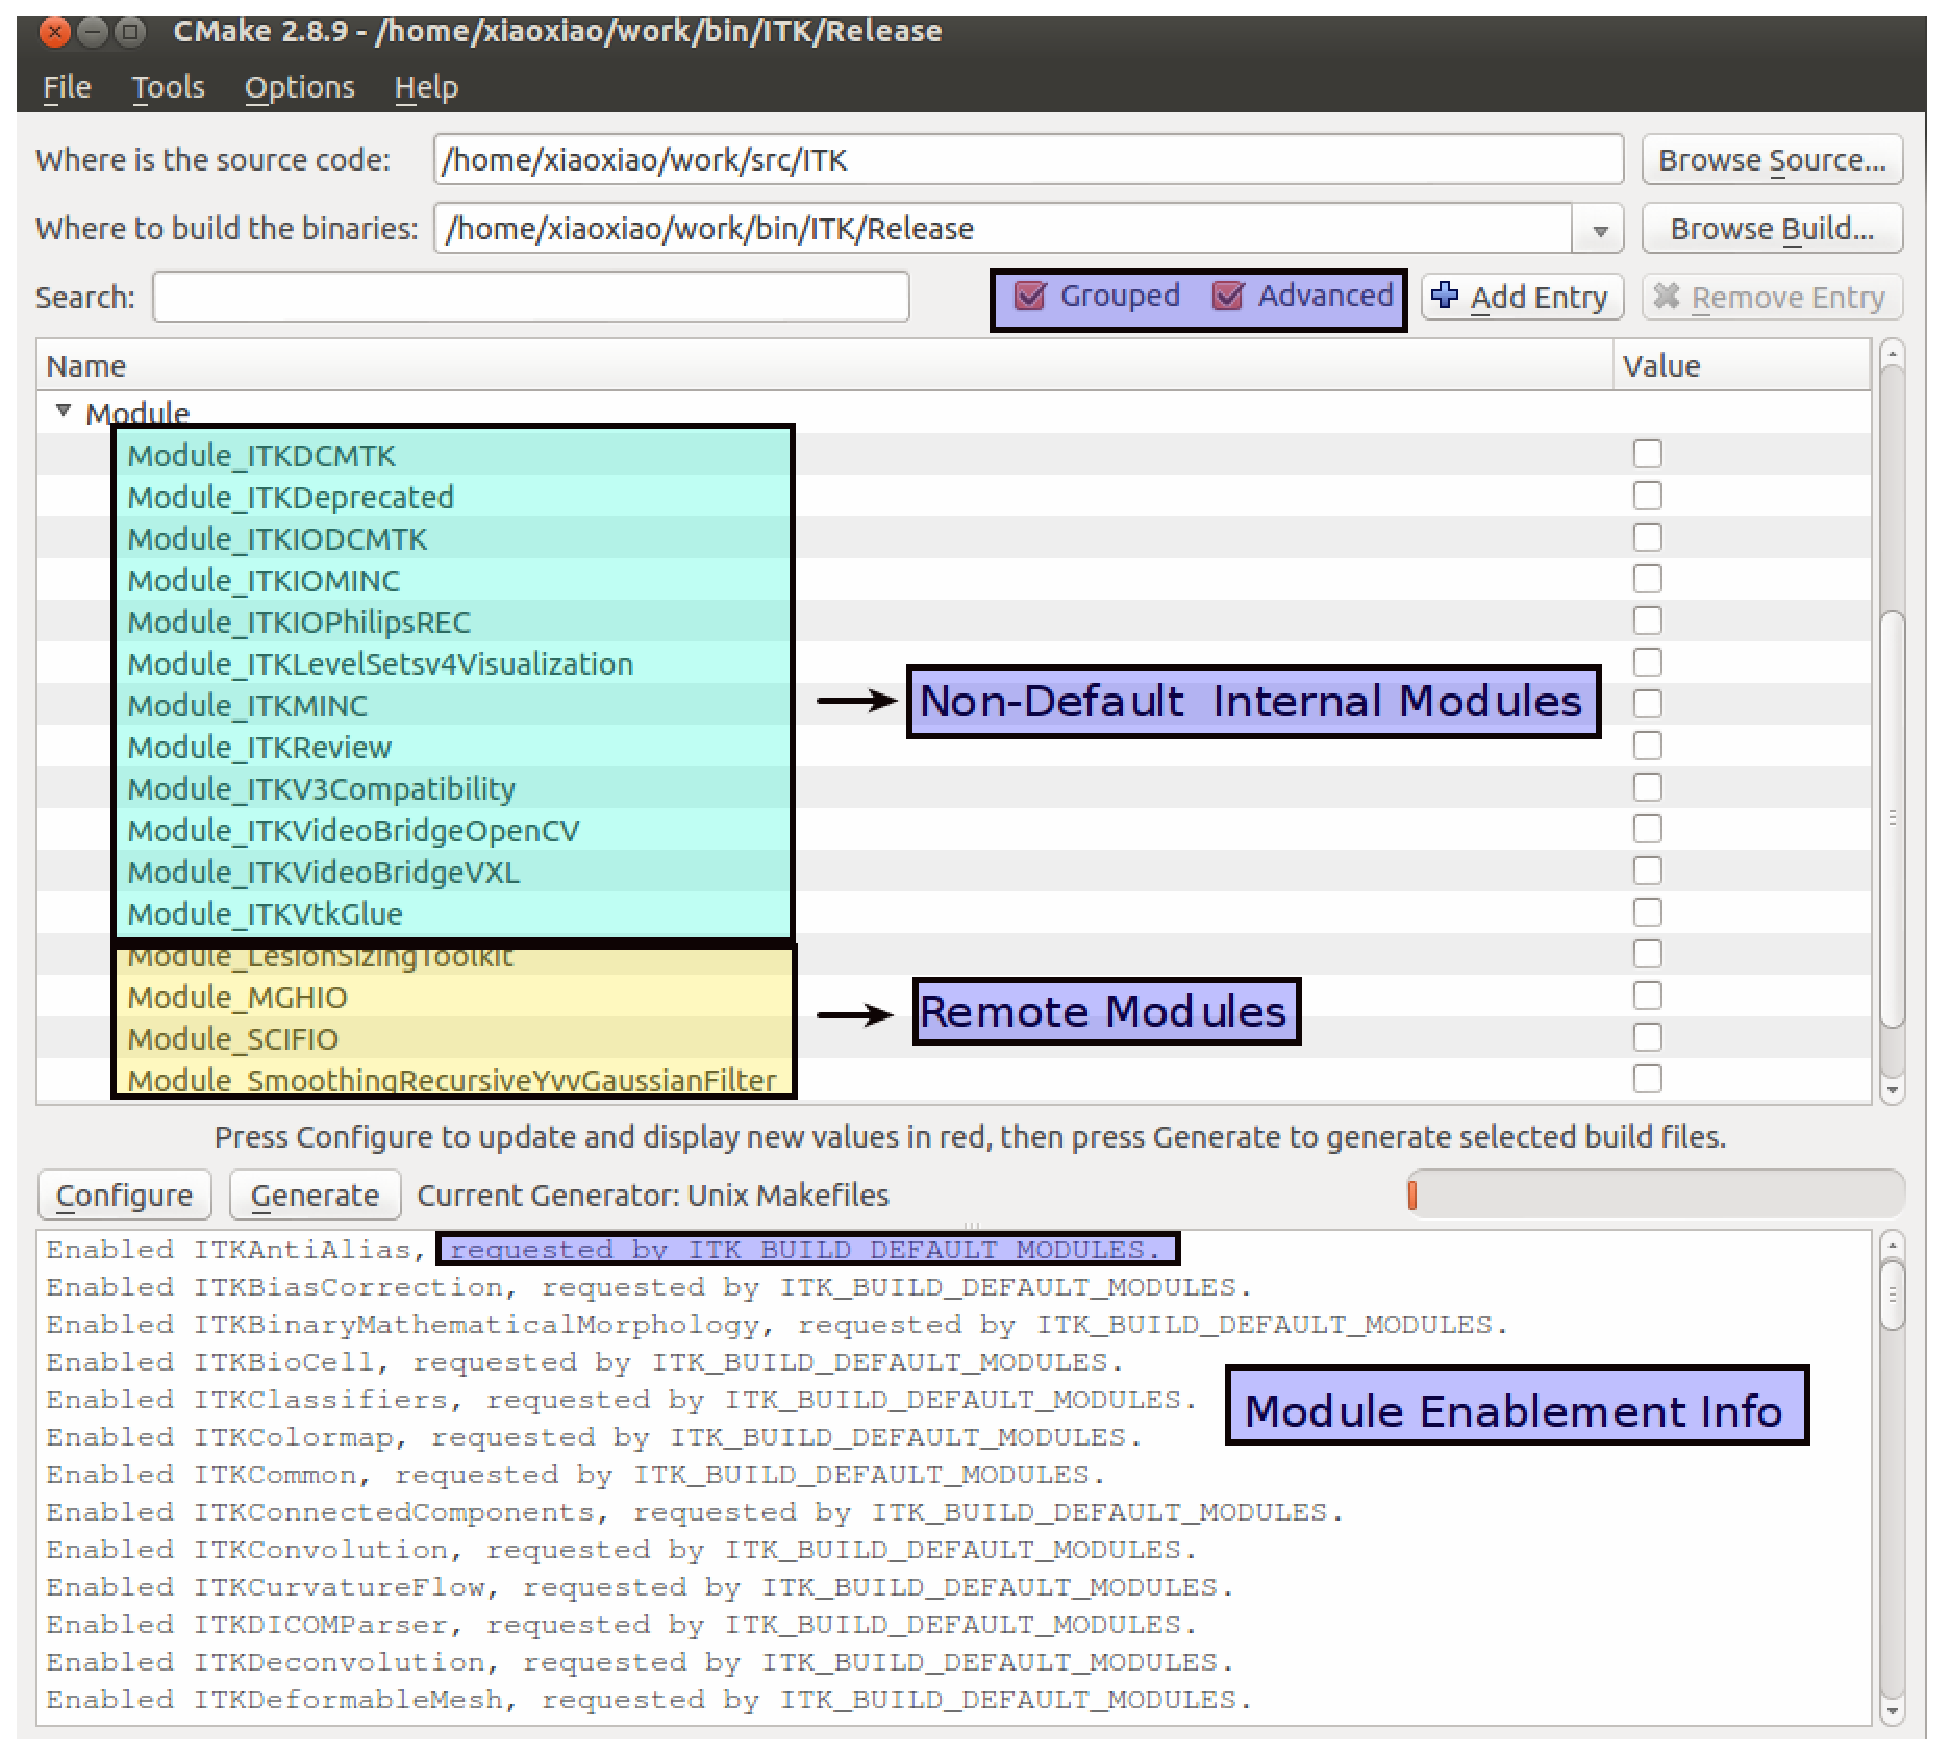
\includegraphics[width=0.8\textwidth]{Configure_ITK_Default.eps}
\itkcaption[Default ITK Configuration]{CMake GUI for configuring ITK: the
advance mode shows options for non-default ITK Modules.}
\label{fig:ConfigITKDefault}
\end{figure}

When \code{ITK\_BUILD\_DEFAULT\_MODULES} is toggled \code{OFF}, users can then
customize the collection of default modules to be included in the ITK library by
the "Group" and "Module" options.

\code{ITKGroup\_\{group name\}} are visible to toggle when
\code{ITK\_BUILD\_DEFAULT\_MODULES = OFF}. The source code repository is
archived  in  such way so that a group of modules that have close relationships
or similar functionalities stay in one subdirectory.  Currently there are 11
groups (not including the External and Remote groups).  The CMake
\code{ITKGroup\_\{group name\}} option is created for the convenience of
enabling or disabling multiple modules at once. The Core group is turned on by
default, see Figure \ref{fig:ConfigITKGroup}.When a group is ON, all the modules in the group
and their depending modules are enabled. When a group is turned OFF, the
modules in the group, except the ones that are required by other enabled
modules, are OFF.

\begin{figure}[htb!]
\centering
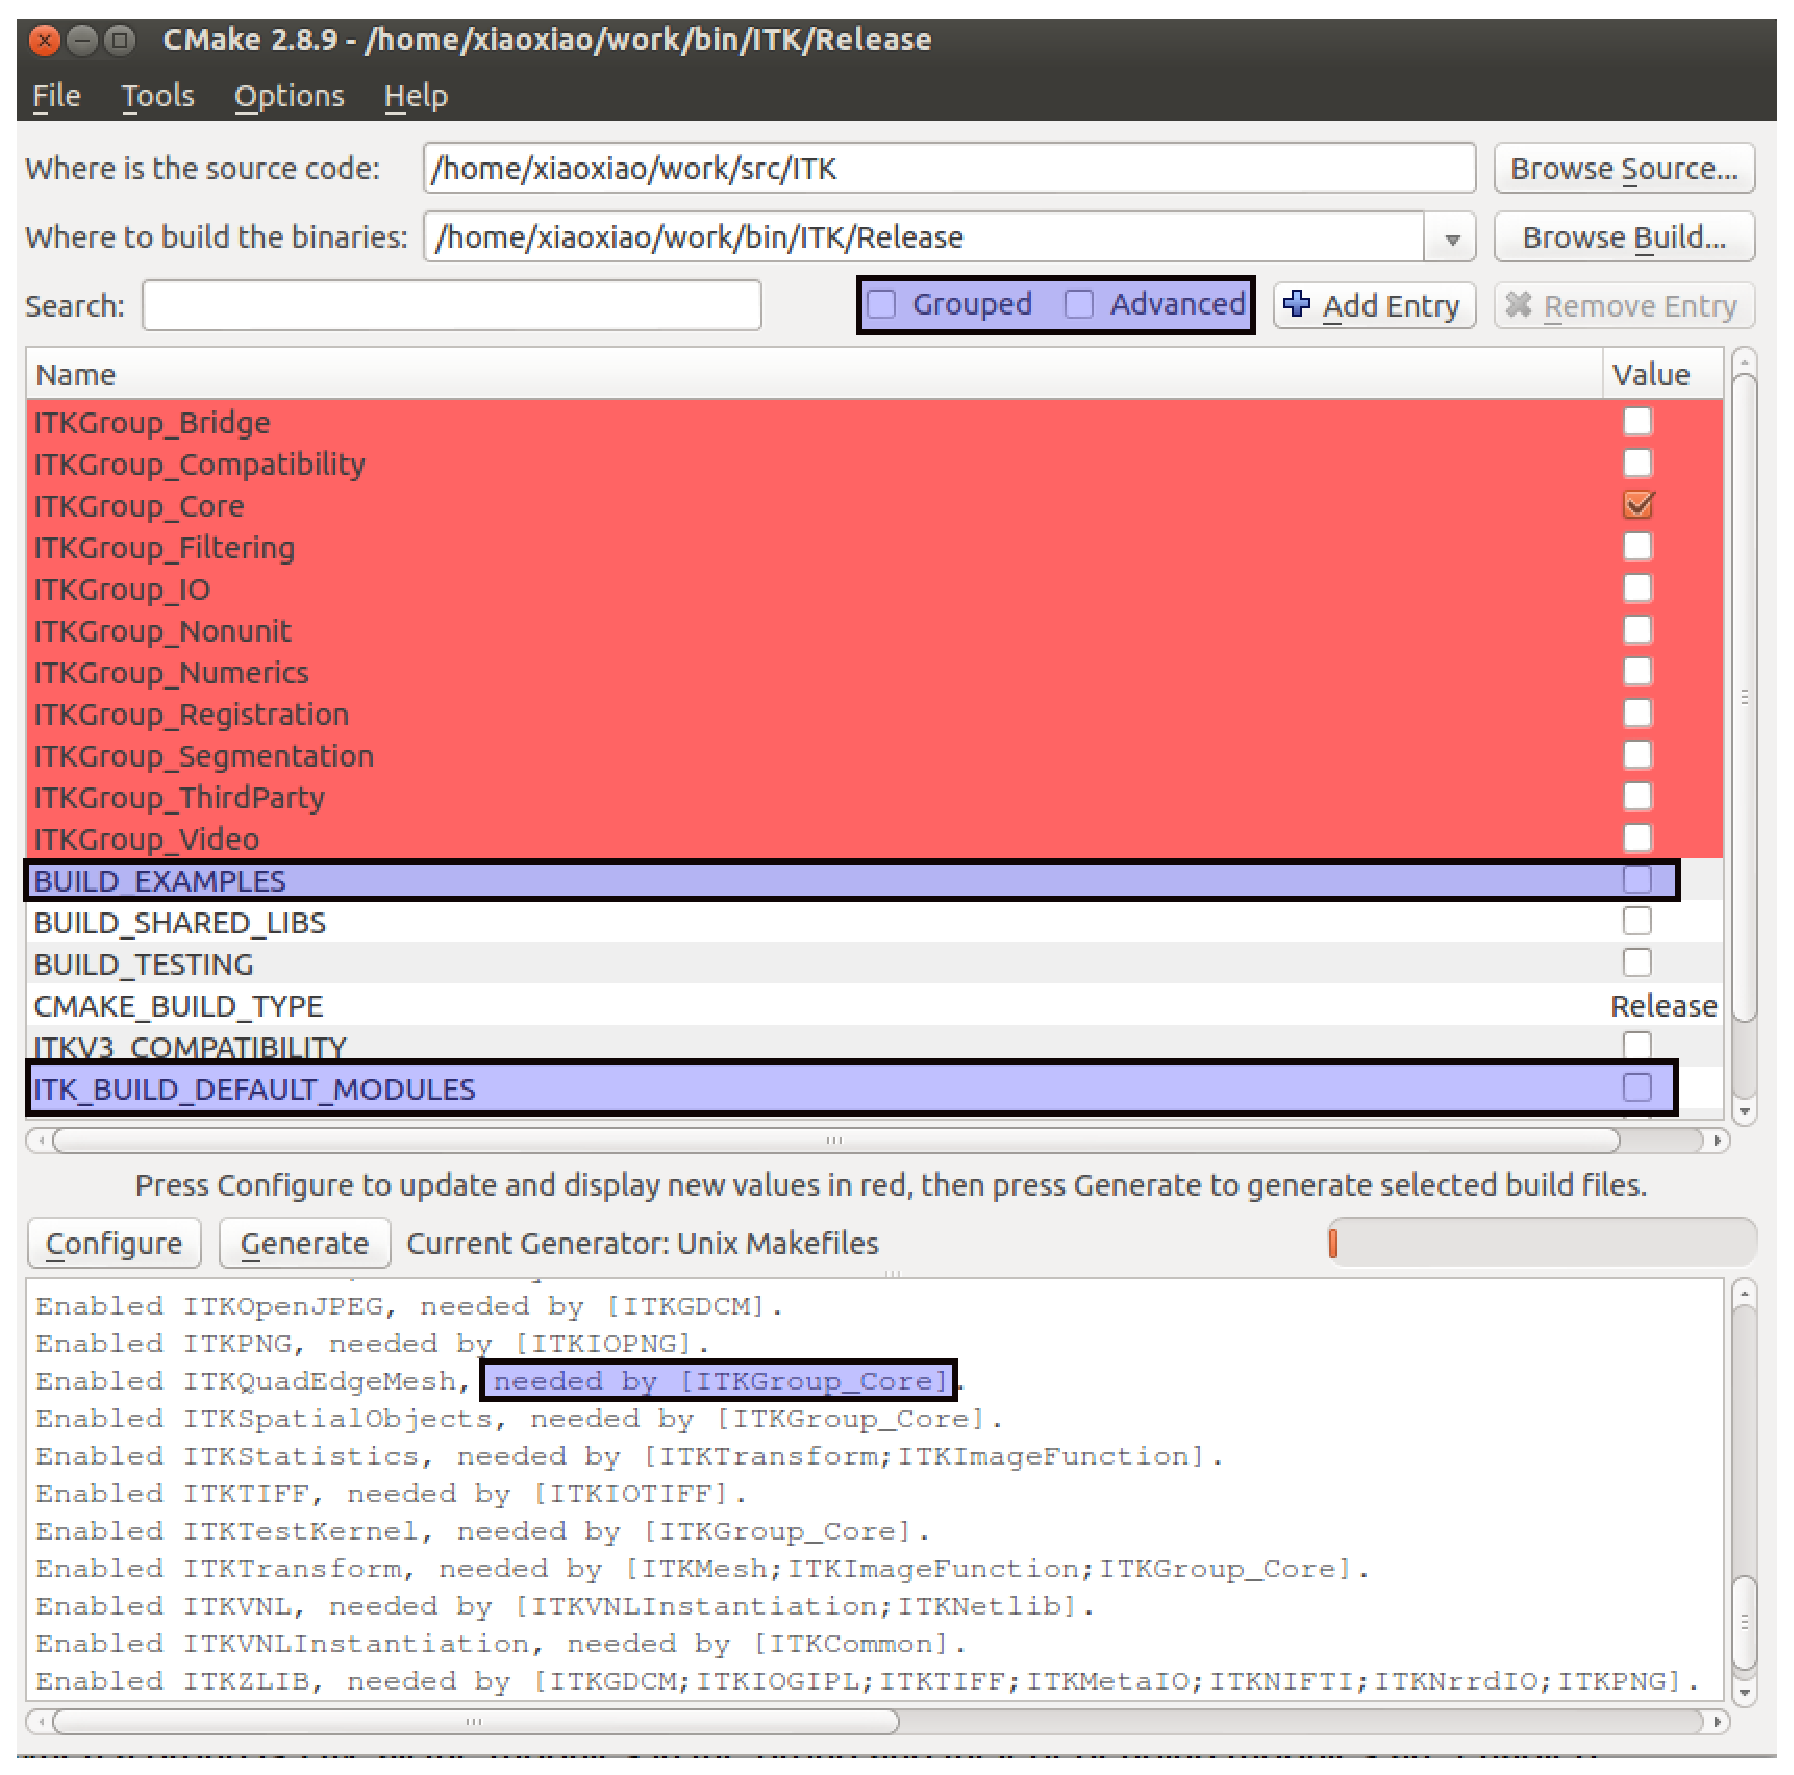
\includegraphics[width=0.8\textwidth]{Configure_ITK_Group.eps}
\itkcaption[ITK Group Configuration]{CMake GUI shows the ITK Group options.}
\label{fig:ConfigITKGroup}
\end{figure}

If you are not sure about which groups to turn on, but you do have a list of
specific modules to be included in your ITK library, you can certainly skip the
Group options and use the \code{Module\_\{module name\}} options only.
Whatever modules you select, their dependent modules are automatically enabled.

However, not all the modules will show up in the GUI for toggle due to the
various levels of controls in the previous two modes.  If they are already
enabled by other modes or enabled by other modules, they will become internal
variable and be hidden from the GUI. For example,  \code{Module\_ITKFoo}
option is hidden for toggle when the module \code{ITKFoo} itself is enabled either  by
1) module dependencies: \code{ITKBar} depends on \code{ITKFoo},   or by 2) the
\code{ITKGroup\_FooAndBar} option: \code{ITKFoo} belongs to the group,  or by 3)
\code{ITK\_BUILD\_DEFAULT\_MODULES=ON} and \code{ITKFoo} is a default module.

To find out why a particular module is enabled, check the CMake configuration
messages where the module enablement information is displayed (Figure
\ref{fig:ConfigITKDefault}). The enablement messages are sorted in alphabetical
order by module names.

\section{Getting Started With ITK }
\label{sec:GettingStartedWithITK}

The simplest way to create a new project with ITK is to create a new directory
somewhere in your disk and create two files in it. The first one is a
\code{CMakeLists.txt} file that will be used by CMake to generate a Makefile
(if you are using UNIX) or a Visual Studio workspace (if you are using
MS-Windows).  The second file is an actual C++ program that will exercise
some of the large number of classes available in ITK. The details of these files
are described in the following section.

Once both files are in your directory you can run CMake in order to configure
your project. Under UNIX, you can \code{cd} to your newly created directory
and type ``\code{ccmake .}''. Note the ``.'' in the command line for
indicating that the \code{CMakeLists.txt} file is in the current directory.
The curses interface will require you to provide the directory where ITK was
built. This is the same path that you indicated for the
\code{ITK\_BINARY\_DIR} variable at the time of configuring ITK. Then CMake
will require you to provide the path to the binary directory where ITK was
built. The ITK binary directory will contain a file named
\code{ITKConfig.cmake} generated during the configuration process at the time
ITK was built.  From this file, CMake will recover all the information
required to configure your new ITK project.

\subsection{Hello World !}
\label{sec:HelloWorldITK}

\index{Hello World}

Here is the content of the two files to write in your new project. These two
files can be found in the \code{ITK/Examples/Installation} directory. The
\code{CMakeLists.txt} file contains the following lines:

% CMake looks similar to bash with regards to formatting.
\begin{minted}[linenos=false]{bash}
project(HelloWorld)

find_package(ITK REQUIRED)
include(${ITK_USE_FILE})

add_executable(HelloWorld HelloWorld.cxx )

target_link_libraries(HelloWorld ${ITK_LIBRARIES})
\end{minted}

The first line defines the name of your project as it appears in Visual
Studio (it will have no effect with UNIX Makefiles). The second line loads a CMake
file with a predefined strategy for finding ITK. If the strategy for finding ITK fails, CMake will prompt
you for the directory where ITK is installed in your system. In that case you
will write this information in the \code{ITK\_BINARY\_DIR} variable. The line
\code{include(\$\{USE\_ITK\_FILE\})} loads the \code{UseITK.cmake} file to set
all the configuration information from ITK. The line \code{add\_executable}
defines as its first argument the name of the executable that will be produced
as result of this project. The remaining arguments of \code{add\_executable}
are the names of the source files to be compiled and linked.  Finally, the
\code{target\_link\_libraries} line specifies which ITK libraries will be
linked against this project.


\input HelloWorld.tex

At this point you have successfully installed and compiled ITK, and created
your first simple program! If you have difficulties, please join the
community mailing list (Section~\ref{sec:JoinMailList} on page
\pageref{sec:JoinMailList}) and pose questions there.
